\documentclass{standalone}

\usepackage{graphicx}
\usepackage{tikz}

\begin{document}



{\small
\begin{tabular}{ *3{c} }
\begin{tikzpicture}
\node[inner sep=0pt, rotate=90] at (0,2)
    {\tiny latitude};
\node[inner sep=0pt] at (2,2)
    {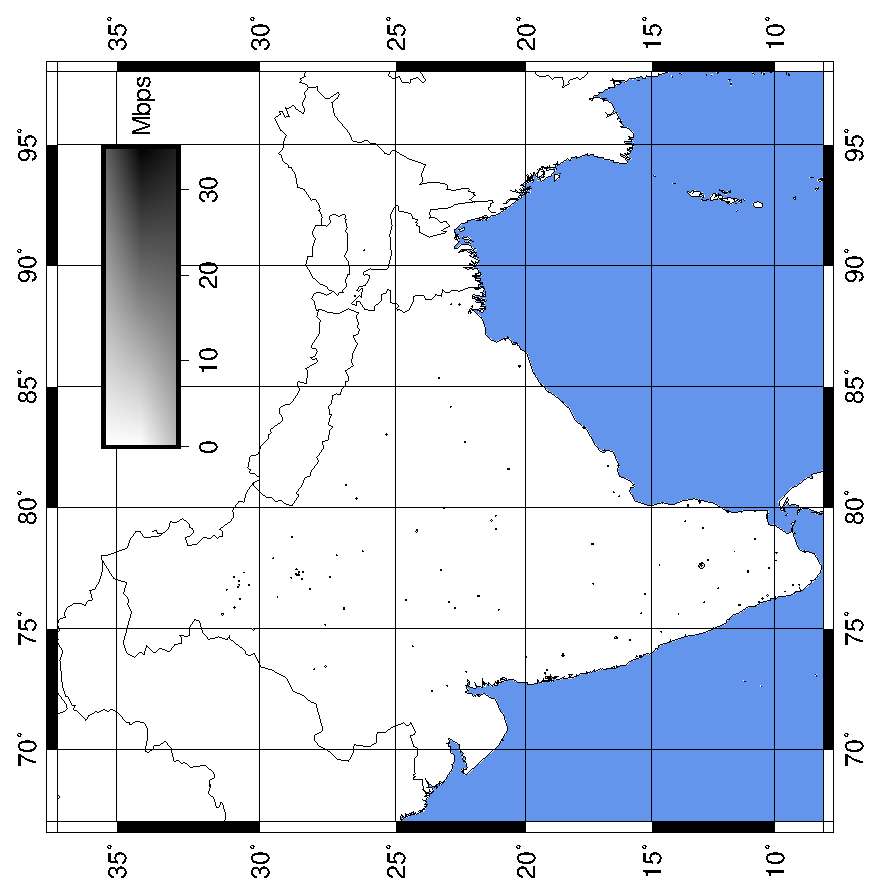
\includegraphics[width=.3\linewidth, angle=270]{2009_09}};
\node[inner sep=0pt] at (2,0)
    {\tiny longitude};
\end{tikzpicture}
  
  & 
  
\begin{tikzpicture}
\node[inner sep=0pt, rotate=90] at (0,2)
    {\tiny latitude};
\node[inner sep=0pt] at (2,2)
    {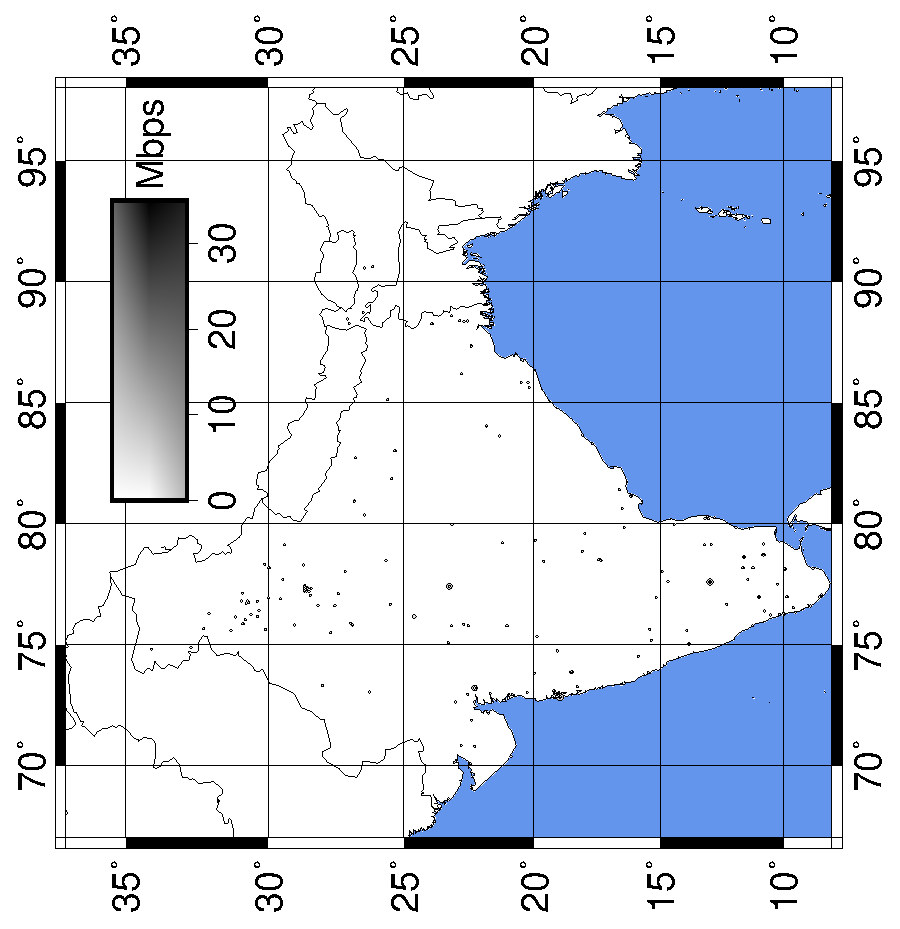
\includegraphics[width=.3\linewidth, angle=270]{2010_09}};
\node[inner sep=0pt] at (2,0)
    {\tiny longitude};
\end{tikzpicture}
  
  & 
  
  
\begin{tikzpicture}
\node[inner sep=0pt, rotate=90] at (0,2)
    {\tiny latitude};
\node[inner sep=0pt] at (2,2)
    {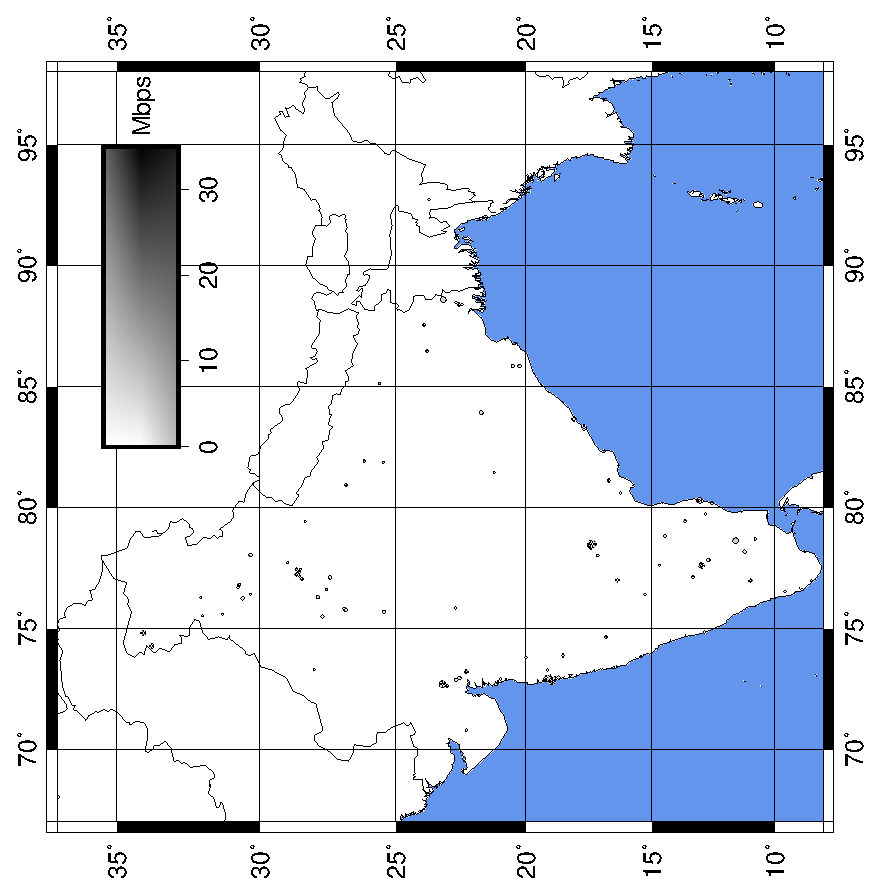
\includegraphics[width=.3\linewidth, angle=270]{2011_09}};
\node[inner sep=0pt] at (2,0)
    {\tiny longitude};
\end{tikzpicture}  
  \\
  (a) September, 2009 & (b) September, 2010 & (c) September, 2011\\[12pt]





\begin{tikzpicture}
\node[inner sep=0pt, rotate=90] at (0,2)
    {\tiny latitude};
\node[inner sep=0pt] at (2,2)
    {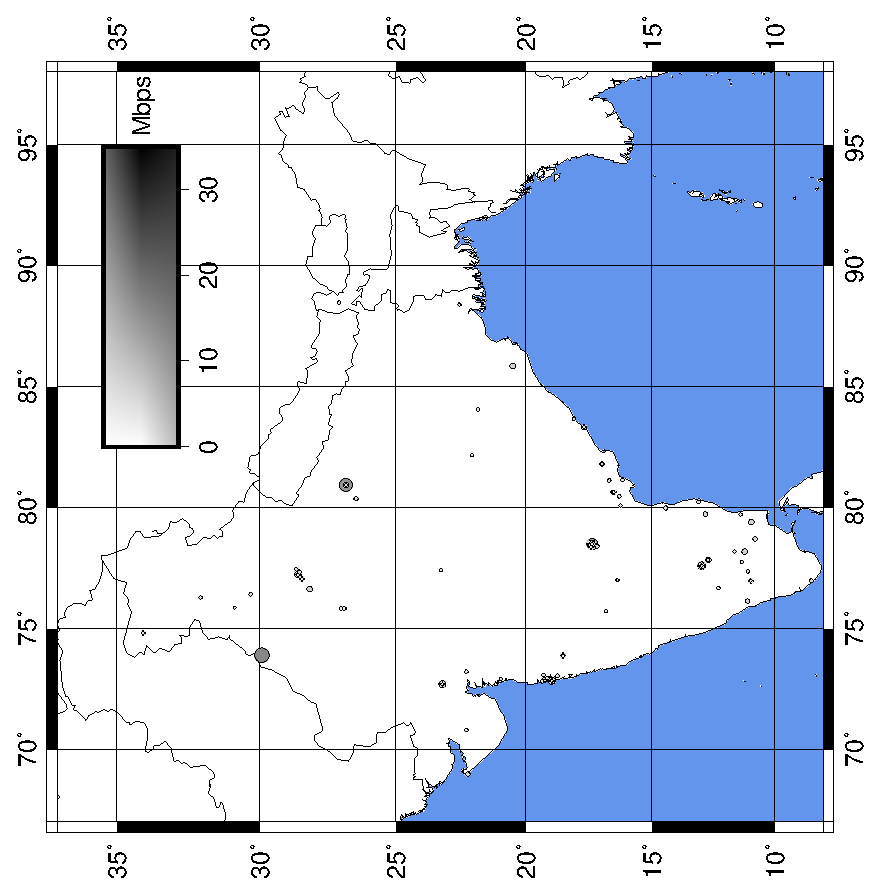
\includegraphics[width=.3\linewidth, angle=270]{2012_09}};
\node[inner sep=0pt] at (2,0)
    {\tiny longitude};
\end{tikzpicture}
  
  & 
  
\begin{tikzpicture}
\node[inner sep=0pt, rotate=90] at (0,2)
    {\tiny latitude};
\node[inner sep=0pt] at (2,2)
    {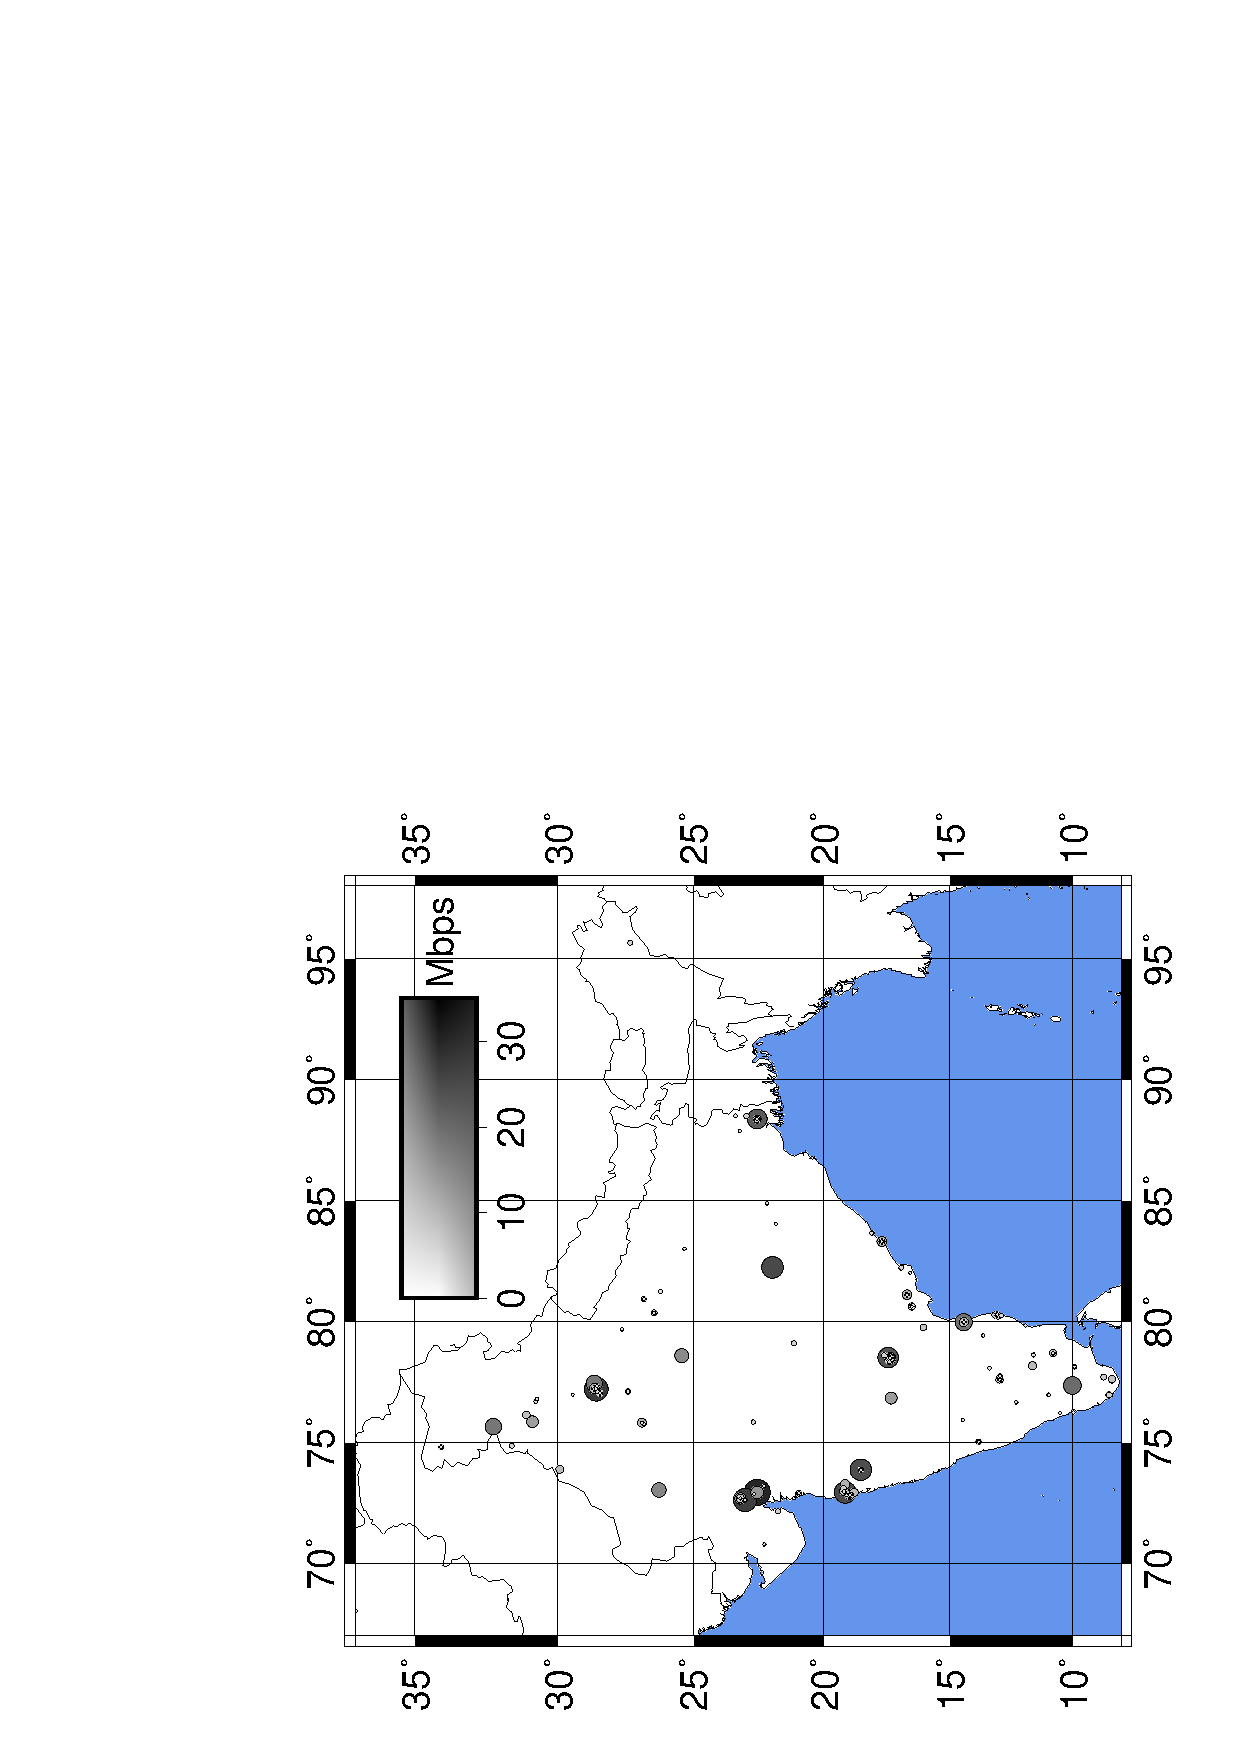
\includegraphics[width=.3\linewidth, angle=270]{2013_09}};
\node[inner sep=0pt] at (2,0)
    {\tiny longitude};
\end{tikzpicture}
  
  & 
  
  
\begin{tikzpicture}
\node[inner sep=0pt, rotate=90] at (0,2)
    {\tiny latitude};
\node[inner sep=0pt] at (2,2)
    {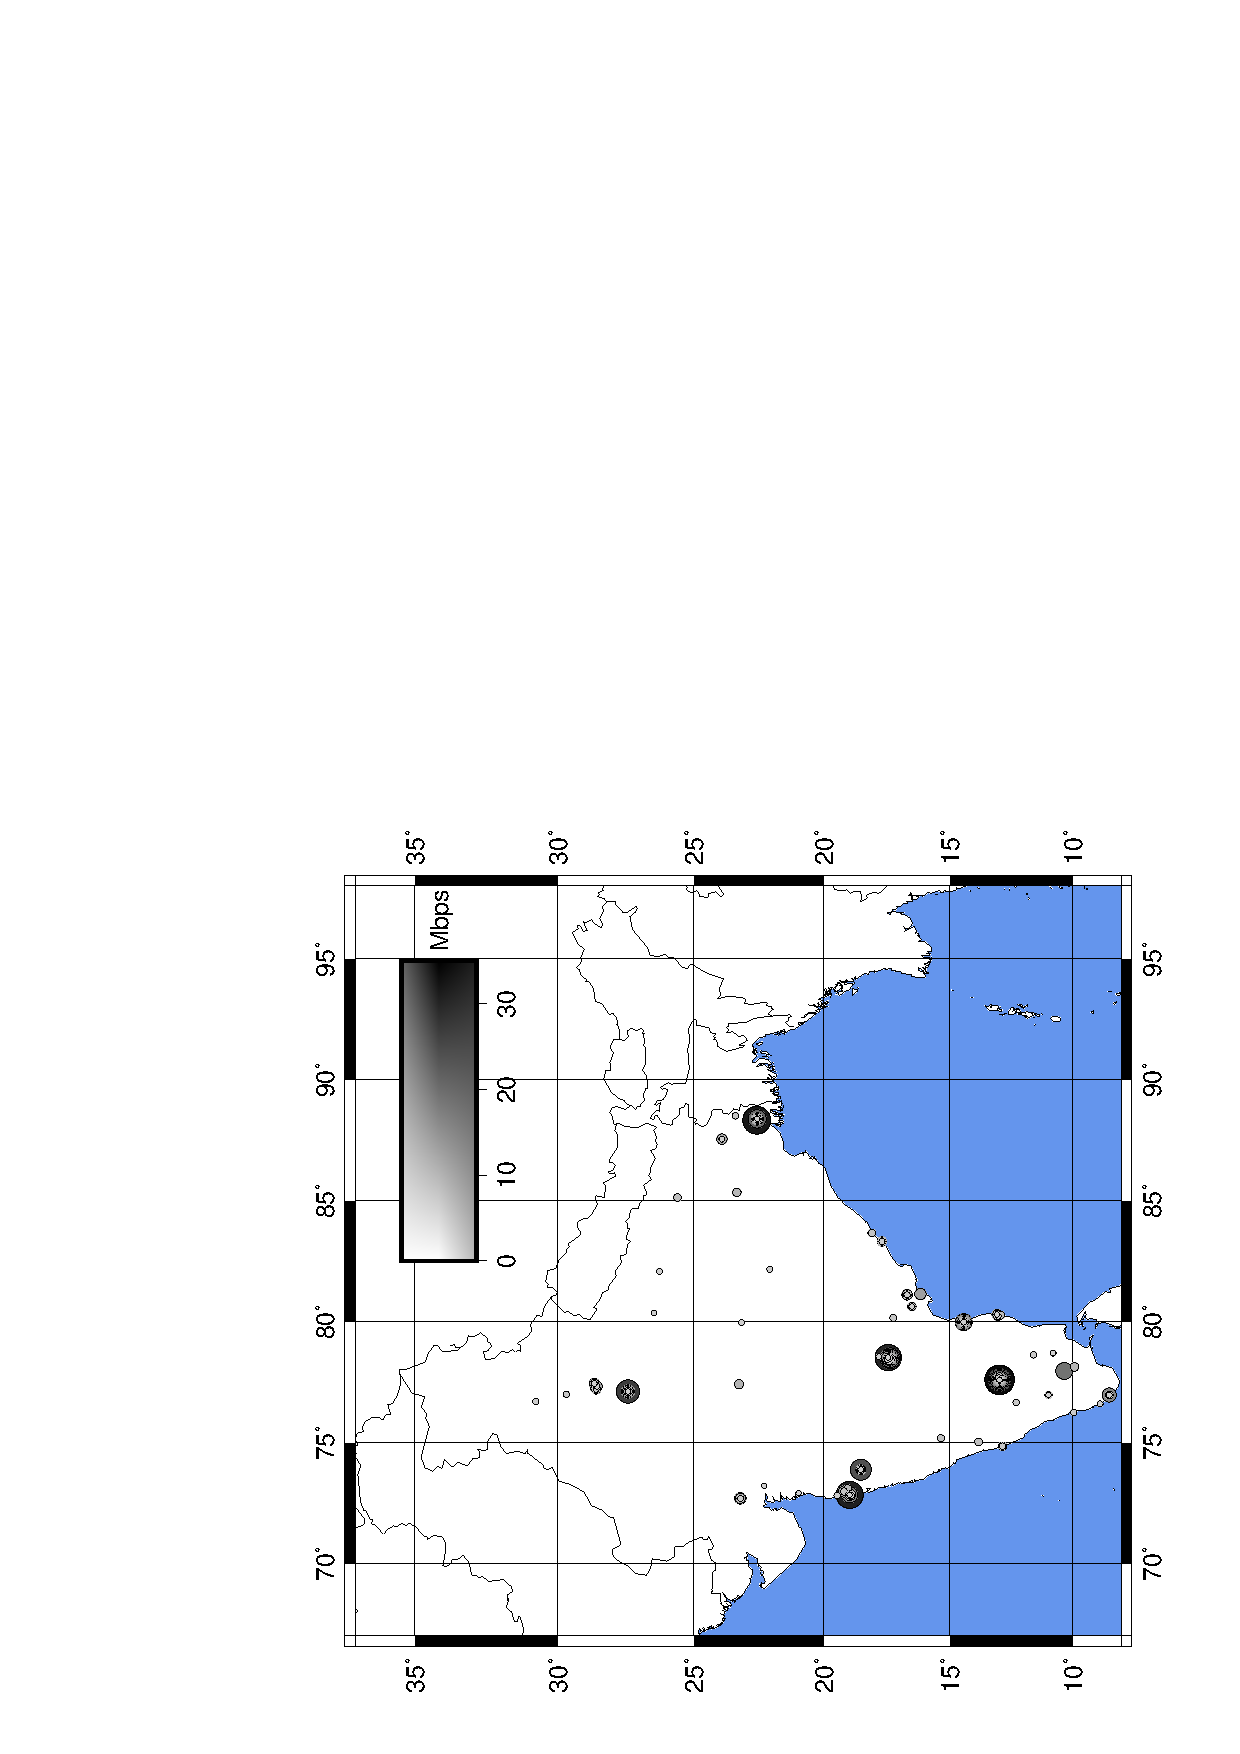
\includegraphics[width=.3\linewidth, angle=270]{2014_09}};
\node[inner sep=0pt] at (2,0)
    {\tiny longitude};
\end{tikzpicture}  
  \\
  (d) September, 2012 & (e) September, 2013 & (f) September, 2014\\

\end{tabular}

}


\end{document}